\documentclass[a4paper]{article}

%% Language and font encodings
\usepackage[english]{babel}
\usepackage[utf8x]{inputenc}
\usepackage[T1]{fontenc}

%% Sets page size and margins
\usepackage[a4paper,top=3cm,bottom=2cm,left=3cm,right=3cm,marginparwidth=1.75cm]{geometry}

%% Useful packages
\usepackage{amsmath}
\usepackage[table,xcdraw]{xcolor}
\usepackage{tabularx,booktabs}
\usepackage{graphicx}
\usepackage[colorinlistoftodos]{todonotes}
\usepackage[colorlinks=true, allcolors=blue]{hyperref}
\usepackage{amsmath}
\usepackage{tikz}
\usepackage{tkz-tab}
\usepackage{caption}
\usepackage{latexsym}
\usepackage{amssymb}
\usepackage{amsmath}
\usepackage{subcaption}
\usepackage{mathtools}
\usepackage{multirow}
\usepackage{listings}
\usepackage{color}
\usepackage{epsfig}
\usepackage{epstopdf}
\usepackage{soul}

%% Useful packages
\usepackage[table,xcdraw]{xcolor}
\usepackage{tabularx,booktabs}
\newcolumntype{C}{>{\centering\arraybackslash}X} % centered version of "X" type
\newcolumntype{b}{X}
\newcolumntype{s}{>{\hsize=.5\hsize}X}
\newcolumntype{v}{>{\hsize=.3\hsize}X}

\definecolor{mygreen}{rgb}{0,0.6,0}
\definecolor{mygray}{rgb}{0.5,0.5,0.5}
\definecolor{mymauve}{rgb}{0.58,0,0.82}


\lstdefinestyle{customc}{
  belowcaptionskip=1\baselineskip,
  breaklines=true,
  frame=L,
  xleftmargin=\parindent,
  language=C,
  showstringspaces=false,
  basicstyle=\footnotesize\ttfamily,
  keywordstyle=\bfseries\color{green!40!black},
  commentstyle=\itshape\color{purple!40!black},
  identifierstyle=\color{blue},
  stringstyle=\color{orange},
}

\lstdefinestyle{customasm}{
  belowcaptionskip=1\baselineskip,
  frame=L,
  xleftmargin=\parindent,
  language=[x86masm]Assembler,
  basicstyle=\footnotesize\ttfamily,
  commentstyle=\itshape\color{purple!40!black},
}

\lstset{escapechar=@,style=customc}

\usetikzlibrary{automata,arrows,positioning,calc}
\usetikzlibrary{shapes,snakes}

% Commands for commenting in inside the text content
\newcommand{\sergio}[1]{\textcolor{brown}{#1}}
\newcommand{\sergiost}[1]{\textcolor{brown}{\st{#1}}}
\newcommand{\franky}[1]{\textcolor{red}{#1}}


%%% TITLE
\title{Komondor User's Guide}
\author{Sergio Barrachina-Mu\~noz and Francesc Wilhelmi}

\begin{document}
\maketitle

\tableofcontents

\listoffigures

\listoftables

%%%%%%%%%%%%%%%
% INTRODUCTION
%%%%%%%%%%%%%%%
\section{Introduction}
\label{section:introduction}

	Komondor \cite{barrachina2017komondor} is an event-based simulator based on COST \cite{chen2002reusing}, and which is mostly intended to reproduce the novel techniques included in the IEEE 802.11ax-2019 amendment \cite{tgax2017draft}.
	
	In this document, we aim to illustrate the installation and execution procedures that must be carried out to successfully perform Komondor simulations. The main goal is therefore to encourage researchers and other practitioners to use the Komondor simulator for their own experiments, and even to participate in the project.	
	
	For more detailed information about the IEEE 802.11-based functionalities that are implemented in Komondor, please refer to \href{https://github.com/wn-upf/Komondor/blob/master/Documentation/Tutorial/LaTeX\%20files/komondor_technical_report.pdf}{this} document.
	
	\textbf{Disclaimer:} Komondor is a project that is constantly evolving, and the contents provided in this document are subject to changes.
	
	%%% Overview
	\subsection{Overview of Komondor}
	\label{section:flowchart}
	Komondor is composed by several modules that allow performing simulations with a high degree of freedom. Here we provide a general overview on the most important module, which are illustrated in Figure \ref{fig:komondor_flowchart}.
	\begin{figure}[h!]
		\centering
		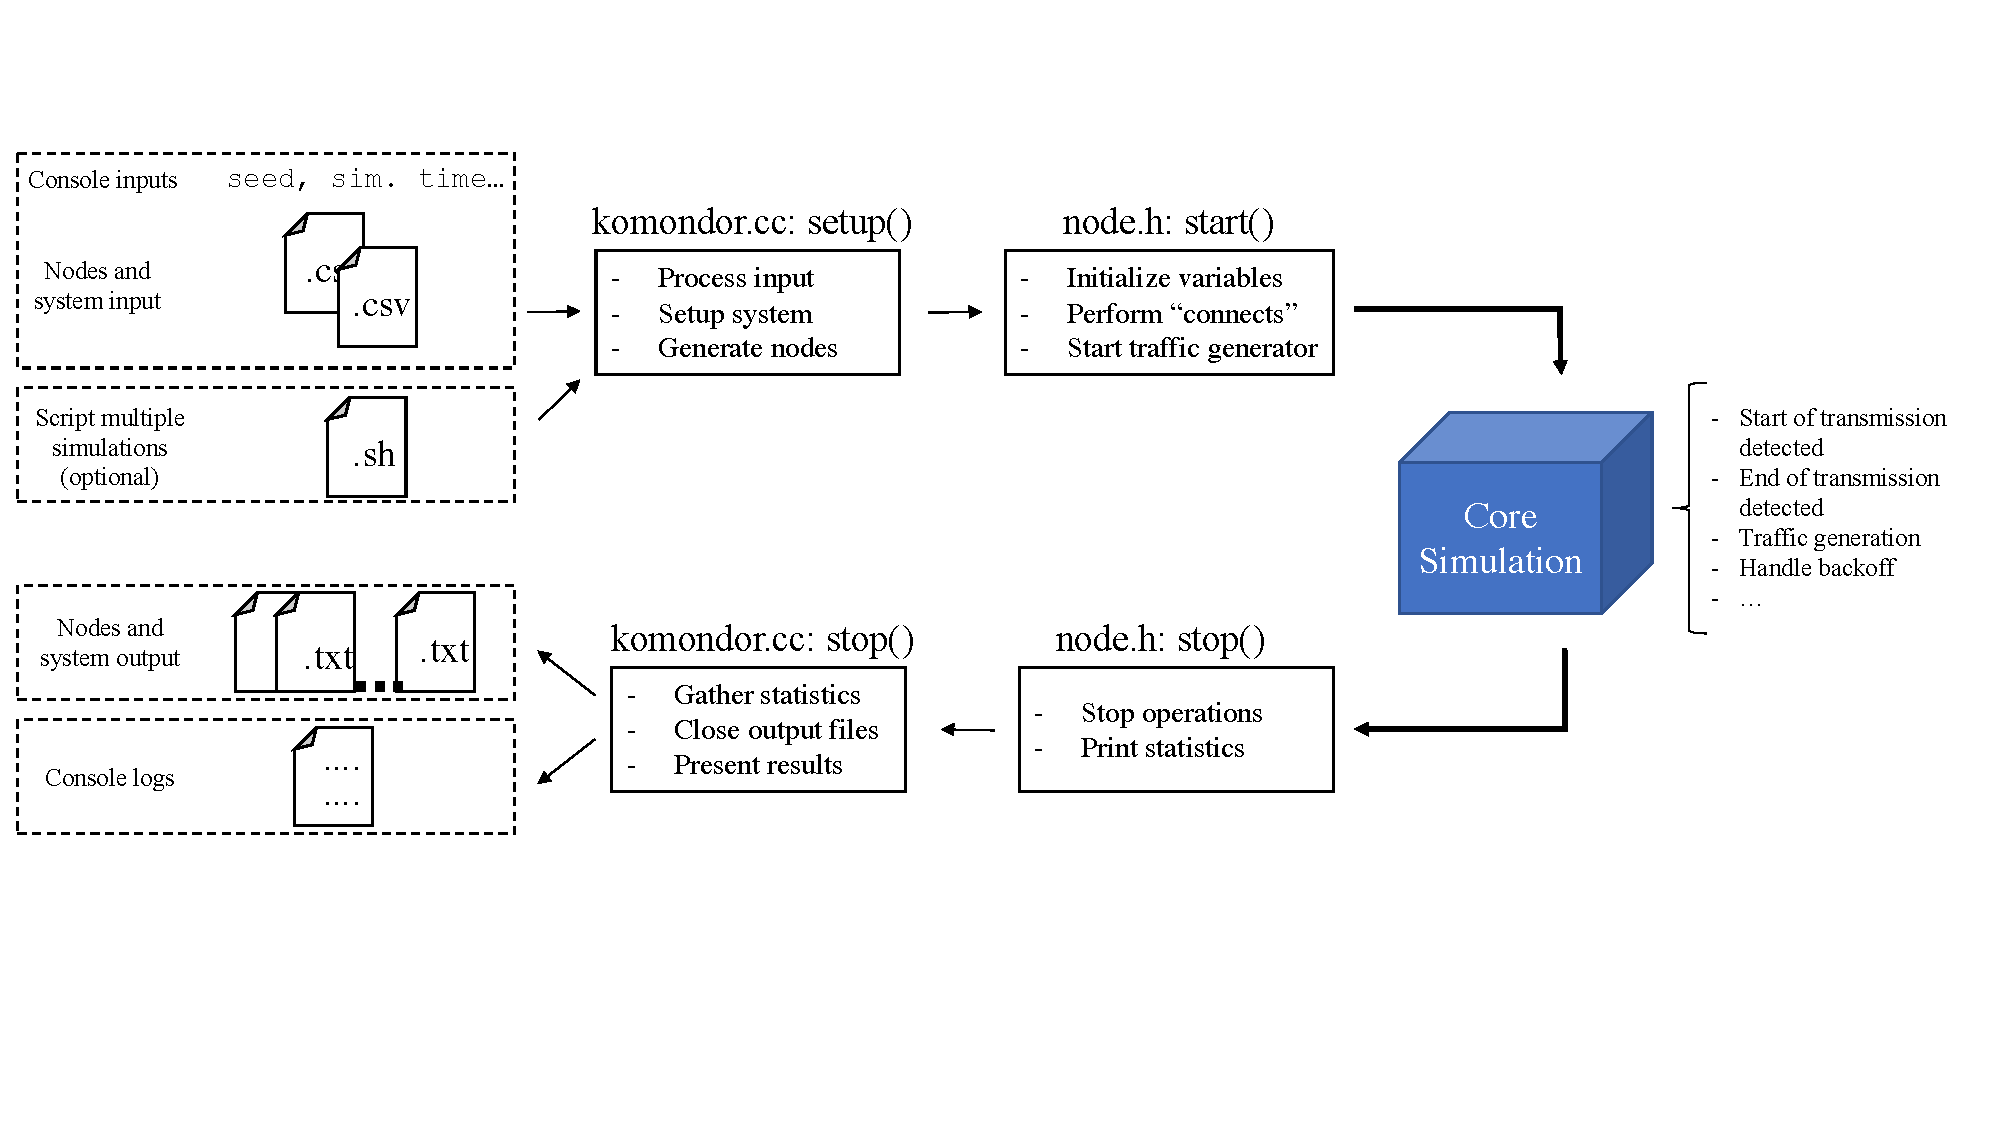
\epsfig{file=images/komondor_flowchart, width=15cm}
		\caption{Komondor flowchart}
		\label{fig:komondor_flowchart}
	\end{figure}		
	
	Komondor receives a set of inputs (information about the nodes, system configuration, simulation time, etc.) and initializes the main module (i.e., \textit{komondor.cc}), which is in charge of generating the network and collecting the information generated within the simulation time. In particular, \textit{komondor.cc} initializes each node in the network (\textit{node.h} components), which act as independent entities and generate data on their own. As a result, during the core simulation, nodes interact among each other by sending packets, so that the DCF operation is implemented for accessing to the channel. Finally, when the simulation runs out (the simulation time is over), a set of outputs are generated with regards to network performance.
	
	The input and output layers are described with more detail later in Sections \ref{section:input} and \ref{section:output}.
	
	% Files organization
	\subsection{Files Organization}
	\label{section:files}		
	To properly understand the Komondor's operation, it is important to know how the project allocated in \href{https://github.com/wn-upf/Komondor}{Github} is organized. In particular, the project is divided into three main folders: \textit{Apps}, \textit{Code} and \textit{Documentation}. \textit{Apps} and \textit{Documentation} folders are intended to contain additional material that supplements the core Komondor's infrastructure (this document, for instance, is inside the \textit{Documentation} folder). Here we focus on the code part, which is organized as follows (refer to Figure \ref{fig:komondor_files} as well):
	\begin{itemize}
		\item \textbf{COST}: constitute the Komondor's primitive operation. Here we find the CompC++ library that allows generating discrete event simulations. For further information about COST, please refer to its main \href{http://www.ita.cs.rpi.edu/cost.html}{website}. 
		\item \textbf{main}: contains the core files (\texttt{komondor.cc}, \texttt{node.h}, \texttt{agent.h} and \texttt{central\_controller.h}) that are in charge of orchestrating all the simulation.  \texttt{komondor.cc} is the main component, which initializes all the other components of \textit{Type II}. All these modules are aware of the existence of the simulation time. In addition to the core components, here we find \texttt{build\_local}, a bash script that compiles the libraries for executing the code. Note that file \texttt{compcxx\_komondor\_main.h} is also required to carry out such a compilation.
		\item \textbf{methods}: by following clean architecture guidelines, independent methods used by core files are contained in the methods folder. Several libraries are provided according to the nature of their functions. For instance, \texttt{backoff\_methods.h} contains methods to handle the backoff operation in DCF.
		\item \textbf{structures}: the Komondor simulator considers several header files to carry out its operation. Among them, we find \texttt{wlan.h}, which defines the main characteristics of a WLAN (WLAN id, list of associated STAs, etc.). In addition, the \texttt{notification.h} structure allows to define the information to be exchanged between devices. 
		\item \textbf{learning\_modules}: here we find the implementation of Machine Learning (ML) methods that receive feedback about the networks performance in simulation time. The utilization of learning mechanisms is further described later in Section \ref{section:input_learning_agents}. 
		\item \textbf{list\_of\_macros.h}: all the static parameters (e.g., constants) are contained in this file.
		\item \textbf{input}: contains the input files that allow building the simulation environment.
		\item \textbf{output}: contains the data generated by Komondor as a result of a given simulation.	
		\item \textbf{scripts\_multiple\_executions}: contains bash scripts to perform multiple simulations.
	\end{itemize} 

	\begin{figure}[h!]
		\centering
		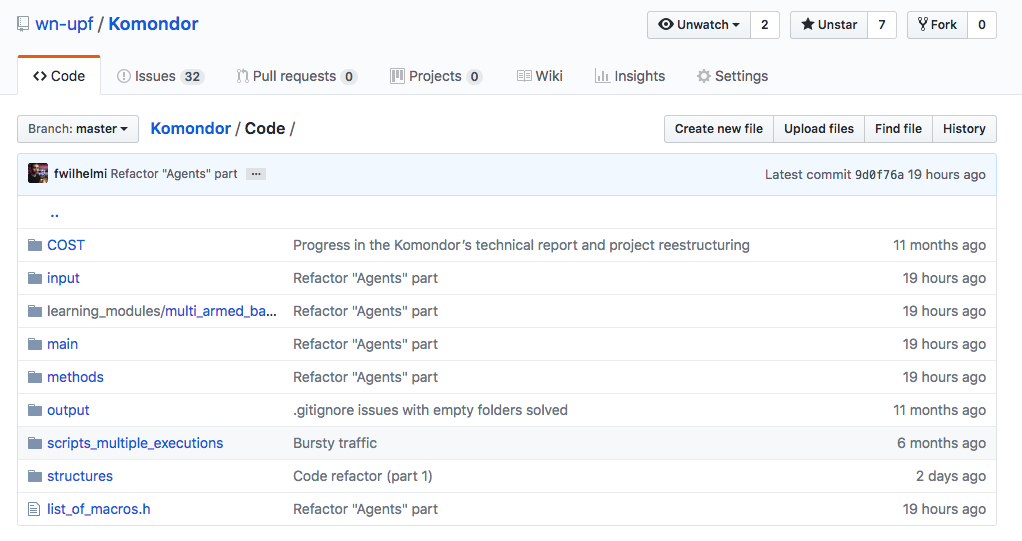
\epsfig{file=images/komondor_files, width=12cm}
		\caption{Komondor files organization}
		\label{fig:komondor_files}
	\end{figure}	

%%%%%%%%%%%%%%%
% INSTALLATION
%%%%%%%%%%%%%%%
\section{Installation}

%%%%%%%%%%%%%%%
% EXECUTION
%%%%%%%%%%%%%%%
\section{Compilation and Execution}
\label{section:execution}
Here we provide the guidelines to properly compile and execute the Komondor simulator. First, we show the execution modes available, and then we describe both the input and the output of the system.

%%% Execution
\subsection{Execution Modes}
\label{section:execution_modes}
To compile and execute Komondor, the following instructions must be followed\footnote{A GNU-based OS is assumed to be used for simulations, including basic compilation programs such as \emph{gcc}.}:
\begin{enumerate}
	\item Set the .csv input files (further defined in Section \ref{section:input})
	\item Access to the "main" directory
	\item Execute "./build\_local". This file contains the instructions for compiling the Komondor code. It has been updated to enable debugging with Valgrind\footnote{Valgrind is a programming tool for memory debugging, memory leak detection, and profiling. Valgrind main website: \url{http://valgrind.org/}}.
	\item Execute \textit{./KomondorSimulator arg\_1 arg\_2 ... arg\_n}, where \textit{arg\_i} is the $i_{\text{th}}$ input argument.
	\item Collect the results either in the output files or in the console.
\end{enumerate}

\textbf{NOTE}: in case that the user does not have permissions to execute some of the files, grant them by introducing the following command in the target folder: \texttt{\$ chmod -R 777 *}.

The execution mode of Komondor depends on the provided input files and the arguments introduced by console. The full list of parameters is described in Table \ref{table:arguments}, and the currently implemented execution modes are summarized below:
\begin{itemize}
	\item \textbf{Basic execution:} simulates the operation of basic WLANs, according to the parameters indicated in the system and nodes input files. Arguments [1, 2, 4, 5, 6, 7, 9, 10, 12, 13] are required for the basic execution.
	\item \textbf{Quick execution:} allows to perform the basic execution by introducing only few parameters. Only the mandatory arguments are required for this kind of execution.
	\item \textbf{Script-based execution:} in this case, the execution is ordered by a bash script, which uses arguments [1, 2, 5, 12, 13].
	\item \textbf{Execution with agents:} in case of including agents, additional parameters must be added to inform about the necessary information that enables the creation of agents. In this case, all the arguments are required to be specified at the console.
\end{itemize}
 
 \begin{table}[h!]
 	\resizebox{\textwidth}{!}{
	\begin{tabular}{|c|c|l|l|}
		\hline
		\textbf{ID} & \textbf{Type} & \multicolumn{1}{c|}{\textbf{Name}} & \multicolumn{1}{c|}{\textbf{Description}}                                                                  \\ \hline
		1           & Mandatory     & system\_input\_filename            & \begin{tabular}[c]{@{}l@{}}File containing system information (e.g., number of \\ channels available, traffic model, etc.). The file must \\ be a .csv with semicolons as separators.\end{tabular}  \\ \hline
		2           & Mandatory     & nodes\_input\_filename             & \begin{tabular}[c]{@{}l@{}}File containing nodes information (e.g., position, \\ channels allowed, etc.). The file must be a .csv with \\ semicolons as separators.\end{tabular}                    \\ \hline
		3           & Optional      & agents\_input\_filename            & \begin{tabular}[c]{@{}l@{}}File containing agents information (e.g., WLAN id, \\ method to execute, possible actions, etc.). The file \\ must be a .csv with semicolons as separators.\end{tabular} \\ \hline
		4           & Optional      & script\_output\_filename           & \begin{tabular}[c]{@{}l@{}}Path to the output file to which write results at the \\ end of the execution (if the file does not exist, the \\ system will create it).\end{tabular}                   \\ \hline
		5           & Optional      & simulation\_code                   & Code provided to a specific simulation.                                                                                                                                                             \\ \hline
		6           & Optional      & save\_system\_logs                 & \begin{tabular}[c]{@{}l@{}}Flag to indicate whether to save the system logs \\ into a file (1) or not (0).\end{tabular}                                                                             \\ \hline
		7           & Optional      & save\_node\_logs                   & \begin{tabular}[c]{@{}l@{}}Flag to indicate whether to save the nodes logs \\ into separate files (1) or not (0). If this flag is \\ activated, one file per node will be created.\end{tabular}     \\ \hline
		8           & Optional      & save\_agent\_logs                  & \begin{tabular}[c]{@{}l@{}}Flag to indicate whether to save the agents logs \\ into separate files (1) or not (0). If this flag is \\ activated, one file per agent will be created.\end{tabular}   \\ \hline
		9           & Optional      & print\_system\_logs                & \begin{tabular}[c]{@{}l@{}}Flag to indicate whether to print the system logs \\ (1) or not (0).\end{tabular}                                                                                        \\ \hline
		10          & Optional      & print\_node\_logs                  & \begin{tabular}[c]{@{}l@{}}Flag to indicate whether to print the nodes logs \\ (1) or not (0).\end{tabular}                                                                                         \\ \hline
		11          & Optional      & print\_agent\_logs                 & \begin{tabular}[c]{@{}l@{}}Flag to indicate whether to print the agents logs \\ (1) or not (0).\end{tabular}                                                                                        \\ \hline
		12          & Mandatory     & sim\_time                          & Simulation time in seconds.                                                                                                                                                                         \\ \hline
		13          & Mandatory     & seed                               & Random seed for the experiments.                                                                                                                                                                    \\ \hline
	\end{tabular}}
	 \caption{List of arguments to be passed to Komondor by console.}
	 \label{table:arguments}
 \end{table}

%%% INPUT
\subsection{Input}
\label{section:input}	
The input files allow Komondor to generate the simulation environment. In particular, we find three main types of input files, which are described in the following subsections.

% System
\subsubsection{System input}
\label{section:system_input}
The system input is introduced through a .csv file, and defines global input parameters such as the number of basic channels considered or the propagation models. System input parameters are defined in Table \ref{table:system_parameters}.

%  System input parameters	
\begin{table}[h!]
	\centering
	\begin{scriptsize}
	\begin{tabular}{|c|c|l|}
		\hline
		\textbf{Parameter} & \textbf{Type} & \multicolumn{1}{c|}{\textbf{Description}} \\ \hline
		num\_channels & int & \begin{tabular}[c]{@{}l@{}}Maximum number of frequency channels \\ in the system\end{tabular} \\ \hline
		basic\_channel\_bandwidth & int & Bandwidth for each channel {[}MHz{]} \\ \hline
		pdf\_backoff & int & PDF to compute the backoff () \\ \hline
		pdf\_tx\_time & int & PDF to compute the tx time () \\ \hline
		packet\_length & int & Length of data packets {[}bits{]} \\ \hline
		ack\_length & int & Length of ACK packets {[}bits{]} \\ \hline
		num\_packets\_aggregated & int & Number of packets aggregated per transmission \\ \hline
		path\_loss\_model & int & \begin{tabular}[c]{@{}l@{}}Path-loss model (0: FSPL, 1: Hata, \\ 2: Indoor 1, 3: Indoor 2, 4: TGax scenario 1)\end{tabular} \\ \hline
		capture\_effect & int & Capture Effect Threshold {[}dB{]} \\ \hline
		noise\_level & int & Floor noise level {[}dBm{]} \\ \hline
		adjacent\_channel\_model & int & \begin{tabular}[c]{@{}l@{}}Co-channel interference model \\ (0: without adjacent interference,\\ 1: contiguous adjacent interference, \\ 2: complete adjacent interference)\end{tabular} \\ \hline
		collisions\_model & int & Collisions model (reserved) \\ \hline
		SIFS & int & SIFS period {[}$\mu$s{]} \\ \hline
		constant\_PER & int & Defines a constant Packet Error Rate \\ \hline
		traffic\_model & int & \begin{tabular}[c]{@{}l@{}}Traffic model (0: full buffer, 1: Poisson distr., \\ 2: deterministic distr.)\end{tabular} \\ \hline
		backoff\_type & int & Type of backoff (discrete: 0, continuous: 1) \\ \hline
		rts\_length & int & Length of RTS packets {[}bits{]} \\ \hline
		cts\_length & int & Length of CTS packets {[}bits{]} \\ \hline
		cw\_adaptation & bool & For activating CW adaptation \\ \hline
		pifs\_activated & bool & For activating PIFS \\ \hline
		capture\_effect\_model & int & Capture effect model \\ \hline
	\end{tabular}
	\end{scriptsize}
	\caption{System input parameters description.}
	\label{table:system_parameters}
\end{table}

An example of system input file can be found in the Github repository:  \href{https://github.com/wn-upf/Komondor/blob/master/Code/input/input_example/input_system_conf.csv}{\textit{Komondor/Code/input/input\_example/input\_system\_conf.csv}}.

% Nodes
\subsubsection{Nodes input}
\label{section:nodes_input}	
Each WLAN is built according to the nodes input, which can define both Access Points (APs) and stations (STAs). In particular, the nodes input introduces characteristics such as type of device, location, or implementing features (e.g., DCB policy). There are two ways of generating nodes, which is explicitly indicated to Komondor through the file name:
\begin{itemize}
	\item In case of including the keyword \emph{nodes}, all the devices (both APs and STAs) must be introduced and described.
	\item Otherwise, if including the keyword \emph{aps}, only the APs are defined, so that a set of STAs is randomly generated under certain introduced parameters (e.g., minimum/maximum number of STAs, maximum distance between APs and STA).\footnote{The usage of APs input files is discouraged to the lack of maintenance.}
\end{itemize}

Table \ref{table:nodes_parameters} describes the Nodes input parameters for both \emph{nodes} and \emph{aps} files. 

% Nodes input parameters		
\begin{table}[h!]
	\centering
	\begin{scriptsize}
	\begin{tabular}{|c|c|c|l|}
		\hline
		\textbf{Parameter} & \textbf{Type} & \textbf{Nodes or APs} & \multicolumn{1}{c|}{\textbf{Description}} \\ \hline
		node\_code & String & nodes & Code assigned to the node \\ \hline
		node\_type & int & nodes & Type of node (0: AP, 1: STA) \\ \hline
		wlan\_code & String & both & Code assigned to the WLAN \\ \hline
		destination\_id & int & nodes & \begin{tabular}[c]{@{}l@{}}To specify the ID of the destination \\ (packets would be only sent to that devices).\\ Setting it to -1 indicates random destination.\end{tabular} \\ \hline
		min\_sta\_number & int & aps & Minimum number of associated STAs \\ \hline
		max\_sta\_number & int & aps & Maximum number of associated STAs \\ \hline
		max\_distance\_sta & int & aps & Maximum distance of associated STAs \\ \hline
		x & int & both & X location {[}m{]} \\ \hline
		y & int & both & Y location {[}m{]} \\ \hline
		z & int & both & Z location {[}m{]} \\ \hline
		primary\_channel & int & both & Primary channel \\ \hline
		min\_channel\_allowed & int & both & Left channel in range \\ \hline
		max\_channel\_allowed & int & both & Right channel in range \\ \hline
		cw & int & both & Fixed CW \\ \hline
		cw\_stage & int & both & Initial CW stage (for CW adaptation) \\ \hline
		tpc\_min & int & both & Minimum transmit power allowed {[}dBm{]} \\ \hline
		tpc\_default & int & both & Default transmit power allowed {[}dBm{]} \\ \hline
		tpc\_max & int & both & Maximum transmit power allowed {[}dBm{]} \\ \hline
		cca\_min & double & both & Minimum CCA allowed {[}dBm{]} \\ \hline
		cca\_default & double & both & Default CCA allowed {[}dBm{]} \\ \hline
		cca\_max & double & both & Maximum CCA allowed {[}dBm{]} \\ \hline
		tx\_antenna\_gain & int & both & Gain of the tx antenna {[}dB{]} \\ \hline
		rx\_antenna\_gain & int & both & Gain of the rx antenna {[}dB{]} \\ \hline
		channel\_bonding\_model & int & both & \begin{tabular}[c]{@{}l@{}}Channel bonding model (0: only primary, \\ 1: SCB, 2: SCB log2, 3: always max, \\ 4: always max log2, 5: always max log2 MCS,\\ 6: uniform probability log2)\end{tabular} \\ \hline
		modulation\_default & int & both & \begin{tabular}[c]{@{}l@{}}Modulation set by default \\ (0 to use dynamic MCS)\end{tabular} \\ \hline
		central\_freq & int & both & Frequency band used (2,4 or 5 GHz) \\ \hline
		lambda & float & both & Packets transmission rate {[}packets/s{]} \\ \hline
		ieee\_protocol & int & both & IEEE protocol used \\ \hline
		traffic\_load & double & both & Traffic load (pkts/s) \\ \hline
	\end{tabular}
	\end{scriptsize}
	\caption{Nodes input parameters description.}
	\label{table:nodes_parameters}
\end{table}

As a final remark, in order to ensure a proper execution, it is mandatory to introduce an input file with a list of nodes ordered by \textit{node\_id} and starting with \textit{node\_id} = 0 (it is a requirement for the array responsible of storing the power perceived by each node). An example of nodes input file can be found in the Github repository:  \href{https://github.com/wn-upf/Komondor/blob/master/Code/input/input_example/input_nodes.csv}{\textit{Komondor/Code/input/input\_example/input\_nodes.csv}}.

% Agents
\subsubsection{Agents input}
\label{section:input_learning_agents}		

Apart from the system and nodes definition, a given user may make use of the learning modules included in Komondor. To that end, the agents input file must be defined, so that specific agents' characteristics (e.g., associated WLAN, learning mechanism or modifiable parameters) are introduced. Table \ref{table:agents_parameters} describes the agents input parameters.

\begin{table}[]
	\begin{scriptsize}
	\begin{tabular}{|c|c|l|}
		\hline
		\textbf{Parameter}      & \textbf{Type} & \multicolumn{1}{c|}{\textbf{Description}}                                                                                                                                     \\ \hline
		wlan\_code              & String        & \begin{tabular}[c]{@{}l@{}}Code corresponding to the WLAN to which the agent is embedded to. \\ Note that the same code must be defined in the nodes input file.\end{tabular} \\ \hline
		centralized\_flag       & int           & \begin{tabular}[c]{@{}l@{}}Flag to indicate whether the node is attached to a centralized system \\ (1) or not (0).\end{tabular}                                              \\ \hline
		time\_between\_requests & double        & Time in seconds between requests performed by the agent to the AP                                                                                                             \\ \hline
		actions\_channels       & int*          & Array of channels available to be selected by the agent.                                                                                                                      \\ \hline
		actions\_cca            & double*       & Array of possible CCA values (in dBm) to be selected by the agent.                                                                                                            \\ \hline
		actions\_tx\_power      & double*       & \begin{tabular}[c]{@{}l@{}}Array of possible transmission power values (in dBm) to be selected \\ by the agent.\end{tabular}                                                  \\ \hline
		actions\_dcb\_policy    & int*          & Array of possible DCB policies to be selected by the agent.                                                                                                                   \\ \hline
		type\_of\_reward        & int           & Type of reward to be used by the agent.                                                                                                                                       \\ \hline
		learning\_mechanism     & int           & Type of learning mechanism to be used by the agent.                                                                                                                           \\ \hline
	\end{tabular}
	\end{scriptsize}
	\caption{Agents input parameters description.}
	\label{table:agents_parameters}
\end{table}

In particular, an agent may act on its own or be part of a centralized system. At the current development stage, the central entity is not fully programmed, and would require from an additional dedicated input file to indicate its operational details. When it comes to the learning mechanisms, so far the \texttt{multi\_armed\_bandits} module is available, which has id 1. Future developments are expected to contemplate the implementation of other Reinforcement Learning (RL) techniques such as Q-learning or Neural Networks. To that end, interactions with other software systems are being contemplated.

An example of agents input file can be found in the Github repository:  \href{https://github.com/wn-upf/Komondor/blob/master/Code/input/input_example/agents.csv}{\textit{Komondor/Code/input/input\_example/agents.csv}}.

% Input scripts
\subsubsection{Input scripts}
\label{section:input_scripts}	
In order to facilitate users work, we provide a set of scripts that allow performing several simulations at once, which is useful to avoid processing different output files. Such sample scripts can be found in the ``scripts multiple executions'' folder, which perform the following operations:
\begin{itemize}
	\item \emph{multiple\_inputs\_script.sh}: processes all the input files contained in ./input/script\_input\_files and generates a simulation for each one. 
	\item \emph{multiple\_inputs\_script\_several\_seeds.sh}: in addition to process multiple inputs, generates different seeds for each simulation.
\end{itemize}

Similar procedures can be implemented to extend the current provided functionalities, such as reading multiple system inputs or generating specific output reports.

%%% OUTPUT
\subsection{Output}
\label{section:output}
The results collected by Komondor can be analyzed after its execution through the generated output. Two information sources are provided: \emph{i)} console logs, and \emph{ii)} logs saved in separated files. The logs generation can be enabled/disabled through the arguments passed to Komondor by console (refer to Section \ref{section:execution_modes}). Note, as well, that major increases in the execution time may occur if logging is activated. For example, for a basic simulation of 4 nodes, simulating 1,000 seconds takes 1.12 s and 15.67 s when not logging and when doing so, respectively.

% Output logs
\subsubsection{Output logs}
\label{section:output_logs}

Komondor, by default, generates a set of console logs regarding the current simulation. For completeness, additional logs can be displayed in relation to node statistics. Such statistics include throughput experienced, collisions, nodes sent, RTS/CTS sent, etc. An example of nodes and system statistics is shown in Figures \ref{fig:nodes_statistics_example} and \ref{fig:general_statistics_example}.

\begin{figure}[h!]
	\centering
	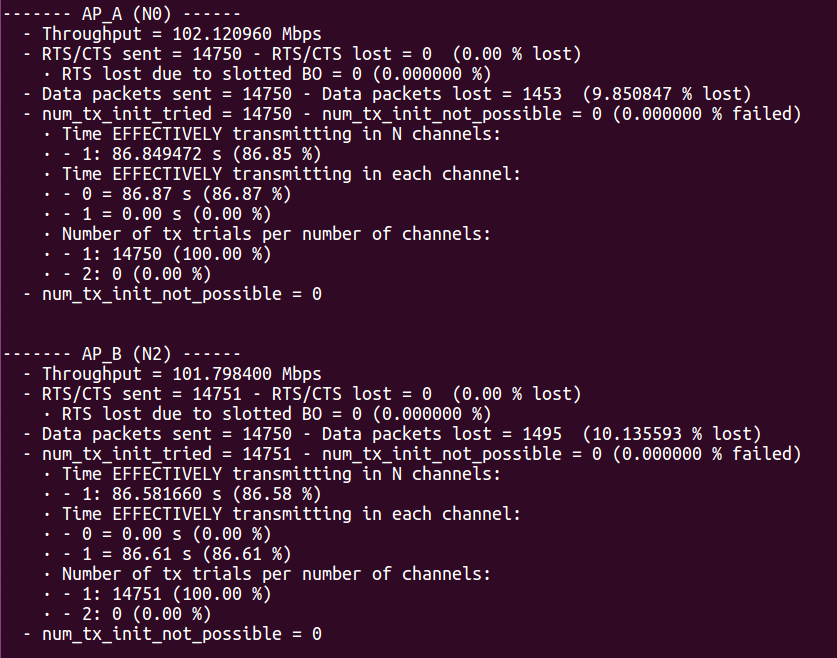
\epsfig{file=images/nodes_statistics_example, width=12cm}
	\caption{Example of nodes statistics in Komondor}
	\label{fig:nodes_statistics_example}
\end{figure}

\begin{figure}[h!]
	\centering
	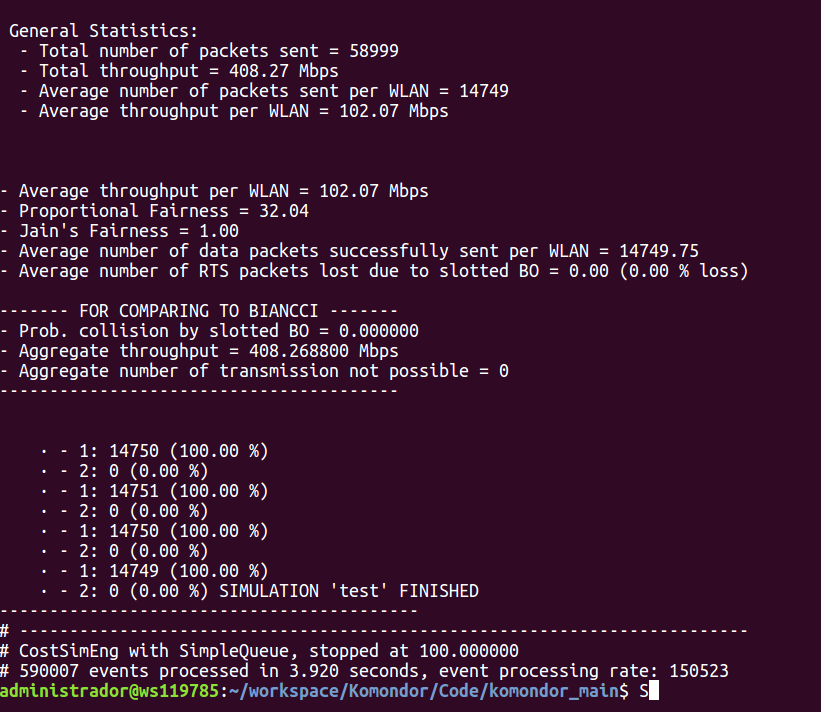
\epsfig{file=images/general_statistics_example, width=12cm}
	\caption{Example of system statistics in Komondor}
	\label{fig:general_statistics_example}
\end{figure}

% Output files
\subsubsection{Output files}
\label{section:output_files}	
Each node can generate logs about its activity, thus describing its IEEE 802.11 operation and the interaction with the other nodes. Such an information is copied into files, which are saved into the \emph{output} folder. In addition agent output files can be generated, thus providing information about the learning procedures.

Finally, in order to make the output files more understandable and classifiable, logs are categorized according to the event that generates it. With that, further filtering processes can be carried out by developers. A potential application may be a network animator. Table \ref{table:event_coding} describes the codes used for each type of event.		
% Events coding table
\begin{table}[h!]
	\centering
	\scriptsize
	\begin{tabular}{|c|c|c|c|}
		\hline
		\textbf{Method}                            & \textbf{Type}       & \textbf{Sub-type} & \textbf{Event description}                              \\ \hline
		Setup()                                    & A                   & -                 & -                                                       \\ \hline
		\multirow{3}{*}{Start()}                   & \multirow{3}{*}{B}  & B00               & Start()                                                 \\ \cline{3-4} 
		&                     & B01               & Start() end                                             \\ \cline{3-4} 
		&                     & B02               & Node's info (one line)                                  \\ \hline
		\multirow{6}{*}{Stop()}                    & \multirow{6}{*}{C}  & C00               & Stop()                                                  \\ \cline{3-4} 
		&                     & C01               & Stop() end                                              \\ \cline{3-4} 
		&                     & C02               & Time transmitting in number of channels                 \\ \cline{3-4} 
		&                     & C03               & Time transmitting in each channel                       \\ \cline{3-4} 
		&                     & C04               & Packets sent                                            \\ \cline{3-4} 
		&                     & C05               & Throughput                                              \\ \hline
		\multirow{14}{*}{inportSomeNodeStartTX()}  & \multirow{14}{*}{D} & D00               & inportSomeNodeStartTX()                                 \\ \cline{3-4} 
		&                     & D01               & inportSomeNodeStartTX() end                             \\ \cline{3-4} 
		&                     & D02               & Node N has started a TX in channels: c\_left - c\_right \\ \cline{3-4} 
		&                     & D03               & Pre update channel state                                \\ \cline{3-4} 
		&                     & D04               & Distance to transmitting node                           \\ \cline{3-4} 
		&                     & D05               & Power received from transmitting node                   \\ \cline{3-4} 
		&                     & D06               & Post update channel state                               \\ \cline{3-4} 
		&                     & D07               & I am (or not) the TX destination                        \\ \cline{3-4} 
		&                     & D08               & Current SINR                                            \\ \cline{3-4} 
		&                     & D09               & Capacitiy                                               \\ \cline{3-4} 
		&                     & D10               & Primary channel affected (or not)                       \\ \cline{3-4} 
		&                     & D11               & Power sensed in primary channel                         \\ \cline{3-4} 
		&                     & D12               & CCA exceeded (or not)                                   \\ \cline{3-4} 
		&                     & D13               & Backoof active (or not)                                 \\ \hline
		\multirow{10}{*}{inportSomeNodeFinishTX()} & \multirow{10}{*}{E} & E00               & inportSomeNodeFinishTX()                                \\ \cline{3-4} 
		&                     & E01               & inportSomeNodeFinishTX() end                            \\ \cline{3-4} 
		&                     & E02               & N\%d has finished a TX in channel range: \%d - \%d      \\ \cline{3-4} 
		&                     & E03               & Initial power of transmitter                            \\ \cline{3-4} 
		&                     & E04               & Pre update channel state                                \\ \cline{3-4} 
		&                     & E05               & Post update channel state                               \\ \cline{3-4} 
		&                     & E06               & Primary channel affected (or not)                       \\ \cline{3-4} 
		&                     & E07               & Power sensed in primary channel                         \\ \cline{3-4} 
		&                     & E08               & CCA exceeded (or not)                                   \\ \cline{3-4} 
		&                     & E09               & I am transmitting (or not)                              \\ \hline
		\multirow{6}{*}{endBackoff()}              & \multirow{6}{*}{F}  & F00               & endBackoff()                                            \\ \cline{3-4} 
		&                     & F01               & endBackoff() end                                        \\ \cline{3-4} 
		&                     & F02               & Channels for transmitting                               \\ \cline{3-4} 
		&                     & F03               & Transmission is possible (or not)                       \\ \cline{3-4} 
		&                     & F04               & Selected transmission range                             \\ \cline{3-4} 
		&                     & F05               & New backoff generated                                   \\ \hline
		\multirow{3}{*}{myTXFinished()}            & \multirow{3}{*}{G}  & G00               & myTXFinished()                                          \\ \cline{3-4} 
		&                     & G01               & myTXFinished() end                                      \\ \cline{3-4} 
		&                     & G02               & New backoff generated                                   \\ \hline
	\end{tabular}
	\caption{Node's event logs encoding}
	\label{table:event_coding}
\end{table}

%%% Example
\subsection{Execution examples}
\label{section:examples}
Here we provide few execution examples with the aim of clarifying the information provided along this section.

\subsubsection{Example 1: Basic execution}
For this simulation, we use the system and nodes input files that can be found at the \href{https://github.com/wn-upf/Komondor/tree/master/Code/input/input_example}{``input\_example''} folder.

The first step is to compile the code through the \texttt{build\_local} file. For that, we access to the ``main'' folder and execute:
\begin{lstlisting}[language=bash,caption={Compling the code}]
	$ cd Komondor/Code/main
	$ ./build_local
\end{lstlisting}

Once the code is compiled without errors, execute the simulation as follows:
\begin{lstlisting}[language=bash,caption={Executing the code}]
$ komondor_main ../input/input_example/system_input.csv ../input/input_example/nodes_input.csv 0 0 1 1 60 789
\end{lstlisting}

In this case, the execution time has been set to 60 seconds and the random seed to 789. File logs have been disabled (the two zeros), but console logs were activated. The results of this simulation can be observed from the console (Figure \ref{fig:example_1_console_output}).

\begin{figure}[h!]
	\centering
	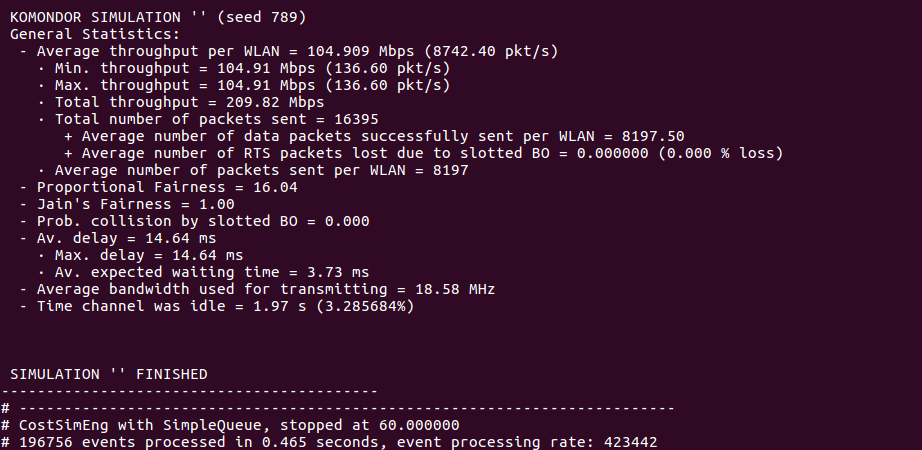
\epsfig{file=images/example_1_console_output, width=12cm}
	\caption{Output logs from example 1.}
	\label{fig:example_1_console_output}
\end{figure}

\subsubsection{Example 2: Execution with agents}
Now, we are showing an execution where intelligent agents are used. For that, we use the same system and input files, and add the agents input file that is located at the same \href{https://github.com/wn-upf/Komondor/tree/master/Code/input/input_example}{folder}. In this case, we use Multi-Armed Bandits (MABs) under an $\varepsilon$-greedy action-selection strategy to allow the WLANs to modify the transmit power and the CCA. For additional details on this implementation, please refer to \cite{wilhelmi2017collaborative}.

Again, we compile the code as before:
\begin{lstlisting}[language=bash,caption={Compling the code}]
$ cd Komondor/Code/main
$ ./build_local
\end{lstlisting}

To execute the simulation, we now introduce more arguments, as described in Section \ref{section:input}.
\begin{lstlisting}[language=bash,caption={Executing the code}]
$ komondor_main ../input/input_example/system_input.csv ../input/input_example/nodes_input.csv ../input/input_example/agents.csv 1 1 1 1 1 1 120 432
\end{lstlisting}

In this occasion, we activated all the types of logs, so the output folder will contain files generated by the system, the nodes and the agents (Figure \ref{fig:output_folder}). Moreover, logs are written at the console, as shown in Figure \ref{fig:example_2_console_output}.

\begin{figure}[h!]
	\centering
	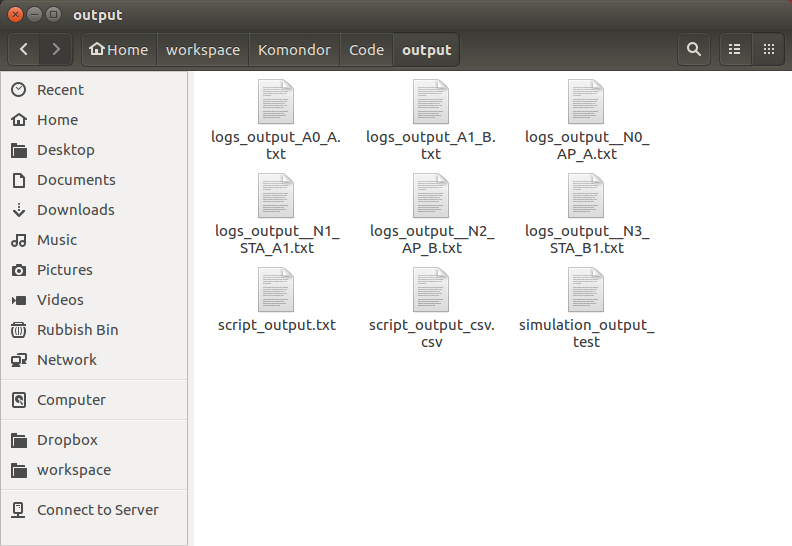
\epsfig{file=images/output_folder, width=12cm}
	\caption{Output files generated in Example 2.}
	\label{fig:output_folder}
\end{figure}

\begin{figure}[h!]
	\centering
	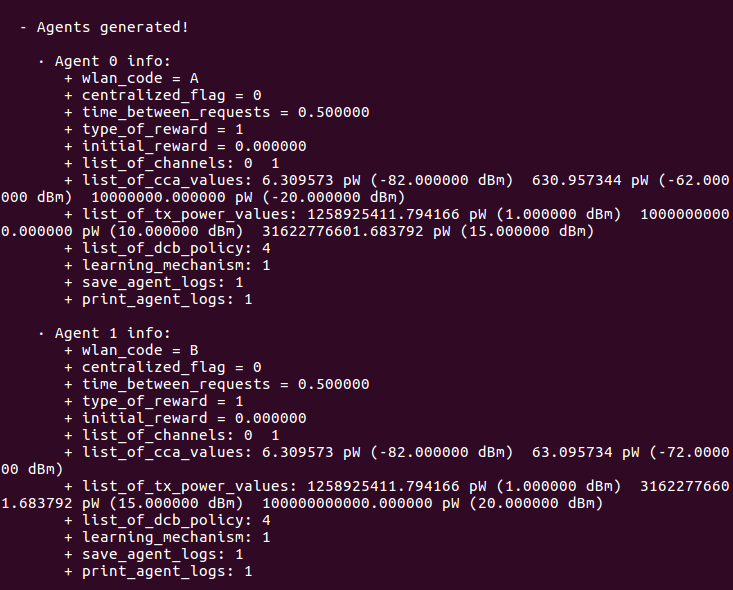
\epsfig{file=images/example_2_console_output, width=12cm}
	\caption{Output logs from Example 2.}
	\label{fig:example_2_console_output}
\end{figure}

%%%%%%%%%%%%%%%
% DEVELOPMENT NOTES
%%%%%%%%%%%%%%%
\section{Development Notes}
Here we provide some clarifications regarding code implementation, wit the aim to facilitate the Komondor's usage and manipulation to developers that may be interested.

%%% Considerations
\subsection{Main considerations}
\label{section:development_considerations}
% TODO: Extend this part.
Some technical information regarding code development is worth to be mentioned to properly understand how to use and modify the Komondor simulator. So far, the main considerations to be taken into account are:		
\begin{itemize}
	\item \textbf{Power and CCA}: power variables are stored in pW (pico watts) in order to be able to operate power magnitudes without loosing resolution\footnote{For instance., the sum of two signals of power values -85 dBm (3.162 pW) and -90 dBm (1 pW), respectively, is -83.803 dBm (4.162 pW).}. However, values are presented to the user in dBm.		
	W (-30)  - mW (0)  - uW (+30) - nW (+60) - pW (+90)\\
	$P_{\text{pw}} = 10^{\frac{P_{\text{dBm}} + 90}{10}}$
\end{itemize}

%%% Miscellany
\subsection{Miscellaneous}
\label{section:development_miscellany}
% TODO: Extend this part.
\begin{itemize}
	\item \textbf{Transmitting capability}: we have added a flag to each node that determines if it is able to transmit (1) or not (0), so that we can decide if the node is only listening or both transmitting and listening.
	\item \textbf{Progress bar}: the Komondor simulation progress bar is displayed through a \textit{printf()} command called by any node with \textit{node\_id} set to 0. If no node has \textit{node\_id} set to 0, the progress bar is not displayed.
\end{itemize}

%%% BIBLIOGRAPHY
\bibliographystyle{unsrt}
\bibliography{bib}

\end{document}